\section*{Math 202A - HW11 - Dan Davison - \texttt{ddavison@berkeley.edu}}

\begin{mdframed}
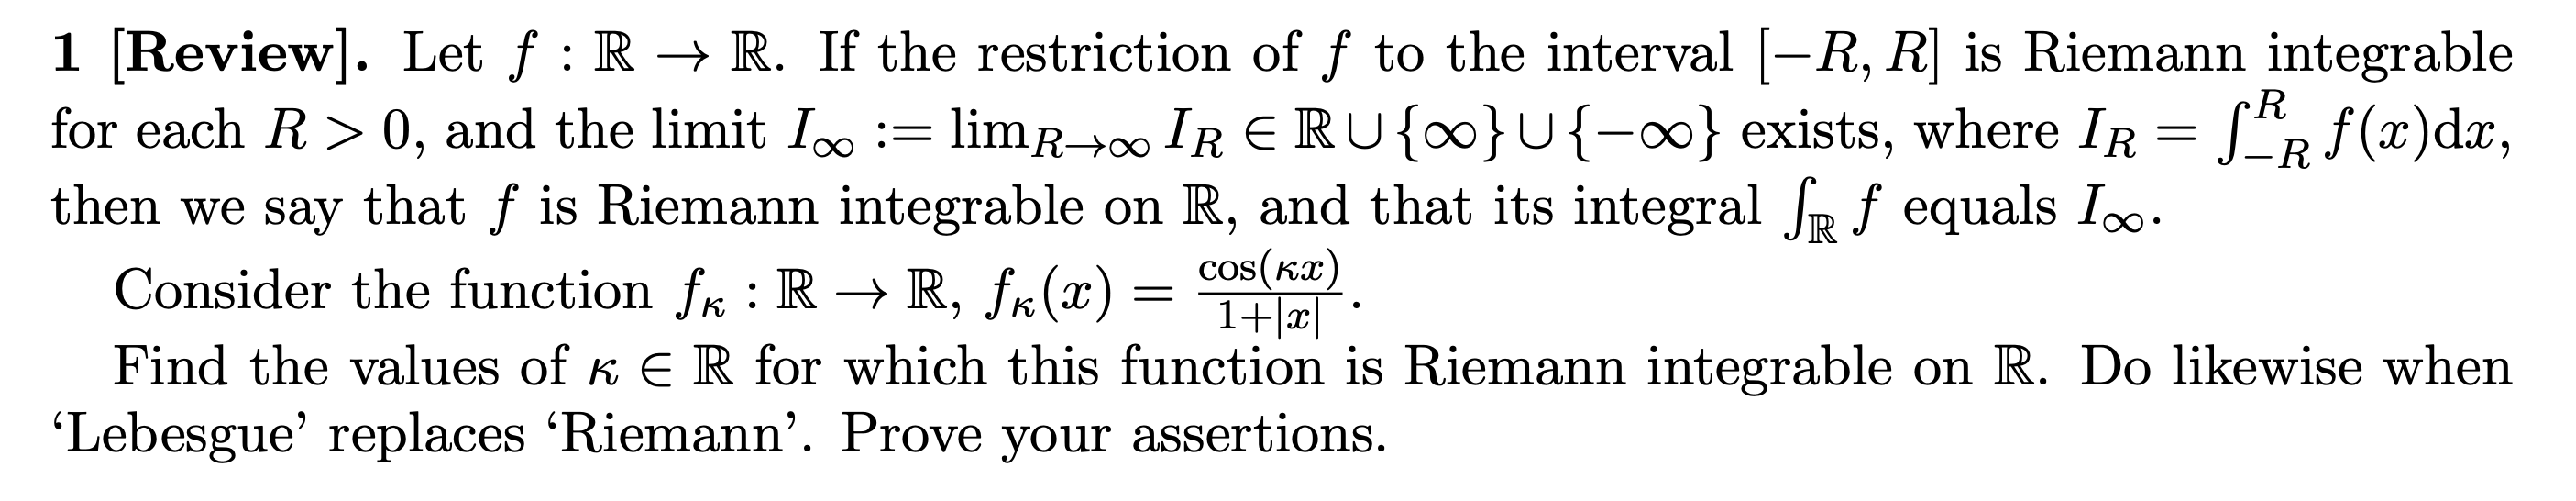
\includegraphics[width=400pt]{img/analysis--berkeley-202a-hw11-8650.png}
\end{mdframed}


\begin{mdframed}
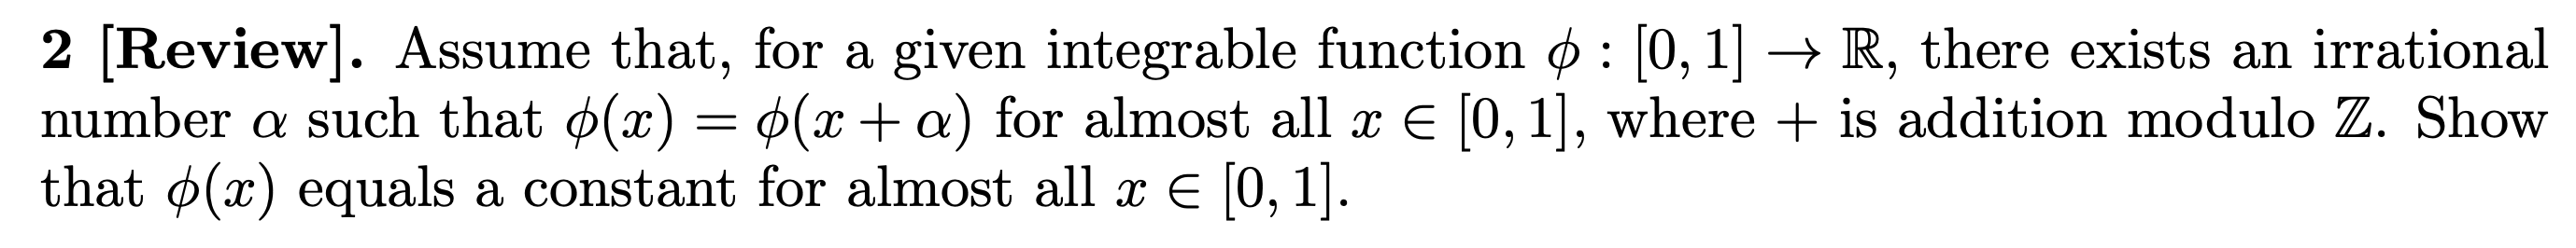
\includegraphics[width=400pt]{img/analysis--berkeley-202a-hw11-b6a3.png}
\end{mdframed}

This is true because the orbit of the map $x \mapsto x + a$ is dense in $[0, 1]$. We basically just need to show that.

We must show that $\phi(x)$ equals a constant for almost all $x$.

Why should that be? Why, for example, can't each orbit have its own constant value?


\begin{proof}
  Let $\tau: [0, 1) \to [0, 1)$ be the map defined by $x \mapsto x + \alpha \mod \Z$, and for $x \in [0, 1)$
  define the sequence $(r_n(x)) = x, \tau(x), \tau^2(x), \ldots$, and
  let $\orb(x) := \big\{r_n(x) ~:~ n \in \N\big\}$ be the orbit of $x$ under $\tau$. Recall from HW2 and HW6
  that for each $x \in [0, 1)$ the sequence $(r_n(x))$ is non-repeating, the corresponding orbit $\orb(x)$ is
  dense in $[0, 1]$, and each orbit is disjoint from every other orbit. Thus each orbit is a countable set and
  there are uncountably many distinct orbits.

  We have that the set of points $x$ at which $\phi(\tau(x)) = \phi(x)$ has measure $1$. Therefore we have the
  following qualitative picture: there are uncountably many disjoint orbits and each orbit is associated with a
  sequence $\phi(x), \phi(\tau(x)), \phi(\tau^2(x)), \ldots$. The set of points at which this sequence changes
  value has measure $0$.

  We must use the fact that $\phi$ is integrable to show that $\phi$ is constant a.e.

  Let $\eps > 0$. According to Lusin's theorem there exists a closed set $F \subseteq [0, 1]$
  with $m(F) > 1- \eps$ such that $\phi|_F$ is continuous. So let $F \subseteq [0, 1]$ be such that $m(F) = 1$
  and $\phi|_F$ is continuous.

  Note that $F$ is uncountable and therefore it contains points from uncountably many orbits.


  Probabilistic view:

  - Pick $x$. It is a member of some orbit and has some value $\phi(x)$. We have $Pr(\phi(x + \alpha) = \phi(x)) = 1$.

  - Suppose the claim is not true. Then there exist $c$ and $d$ such that $m(\phi = c) = p_c > 0$ and $m(\phi = d) = p_d > 0$.

  - Pick $x$. With probability $p_c$ we have $\phi(x) = c$ and also $\phi(x + \alpha) = c$.










  Why might $\phi$ be constant a.e.?

  - Each orbit is countable, so if one orbit is constant, that's just a measure zero set.

  - Similarly, if every orbit is constant, but they all have different values that's not constant a.e.

  - What we need to show is something more like that all orbits ``start​'' with the same value

\end{proof}


\begin{mdframed}
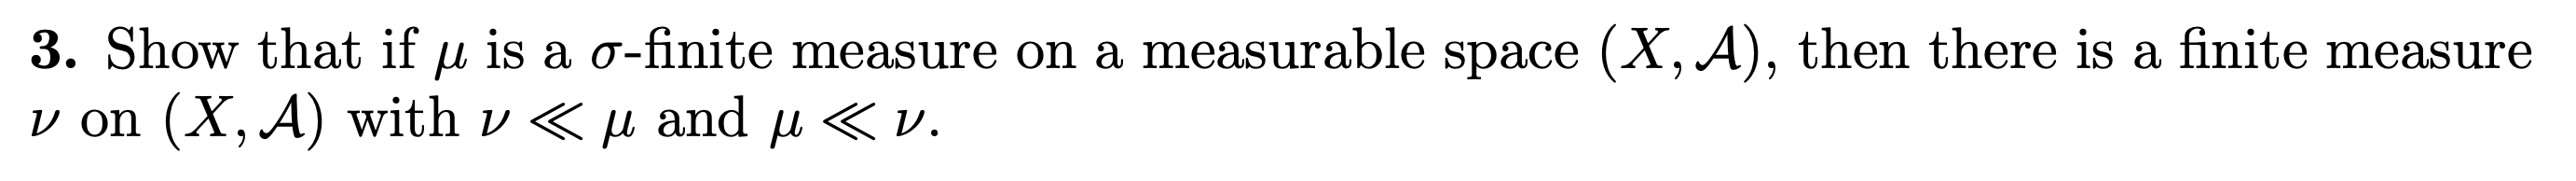
\includegraphics[width=400pt]{img/analysis--berkeley-202a-hw11-3704.png}
\end{mdframed}


\begin{mdframed}
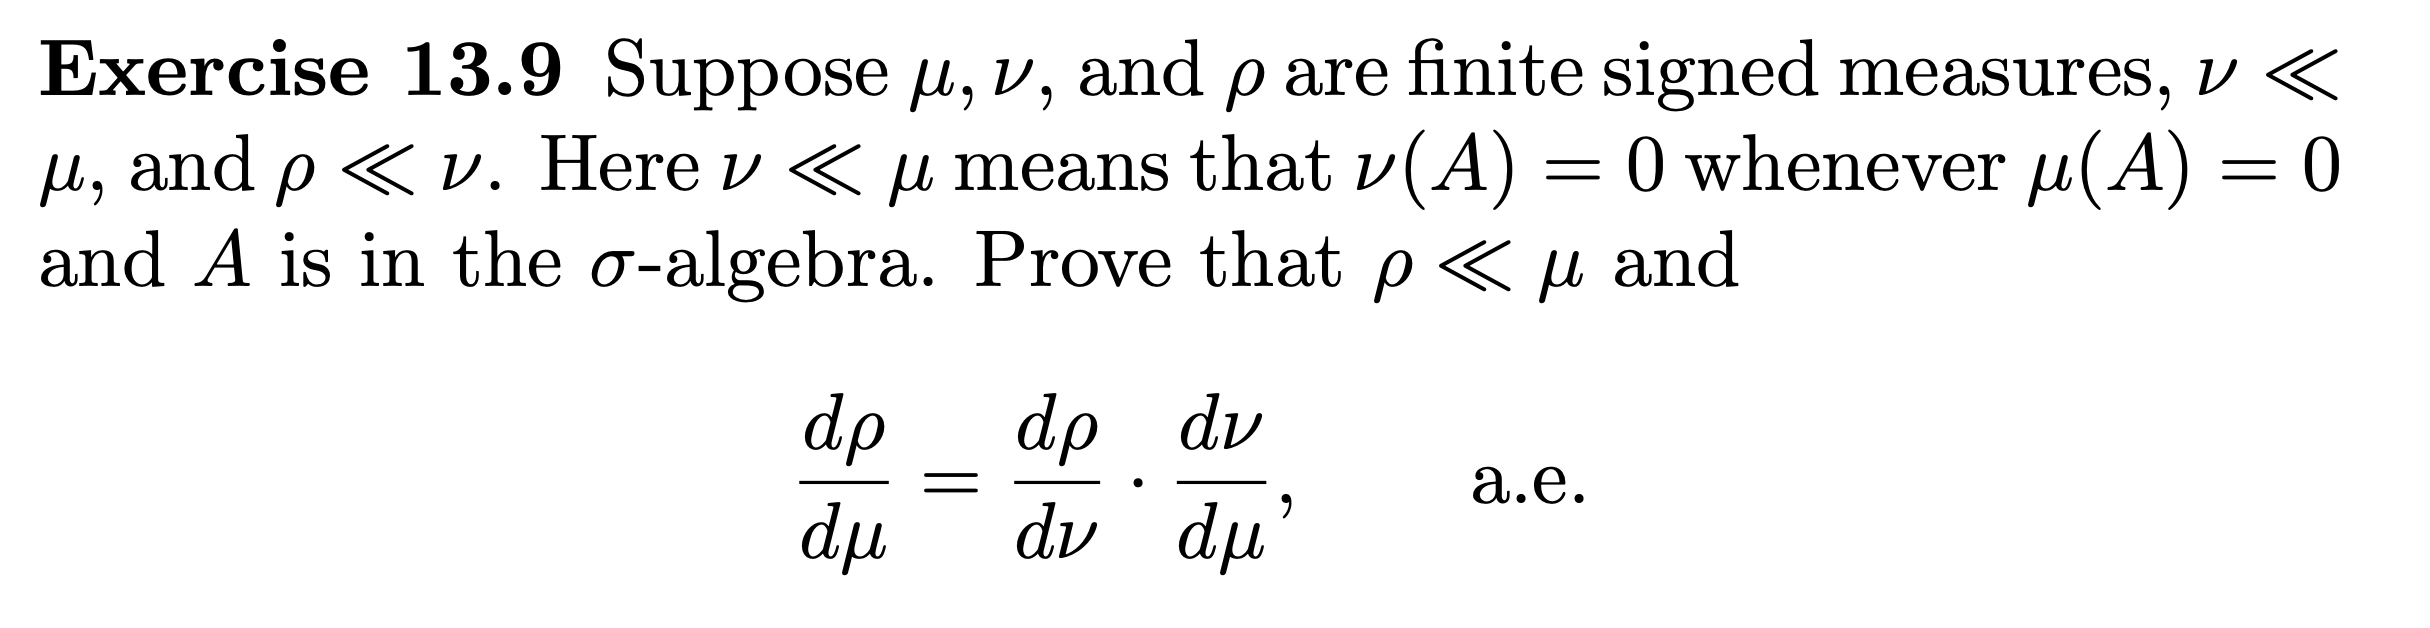
\includegraphics[width=400pt]{img/analysis--berkeley-202a-hw11-f2c0.png}
\end{mdframed}


\begin{mdframed}
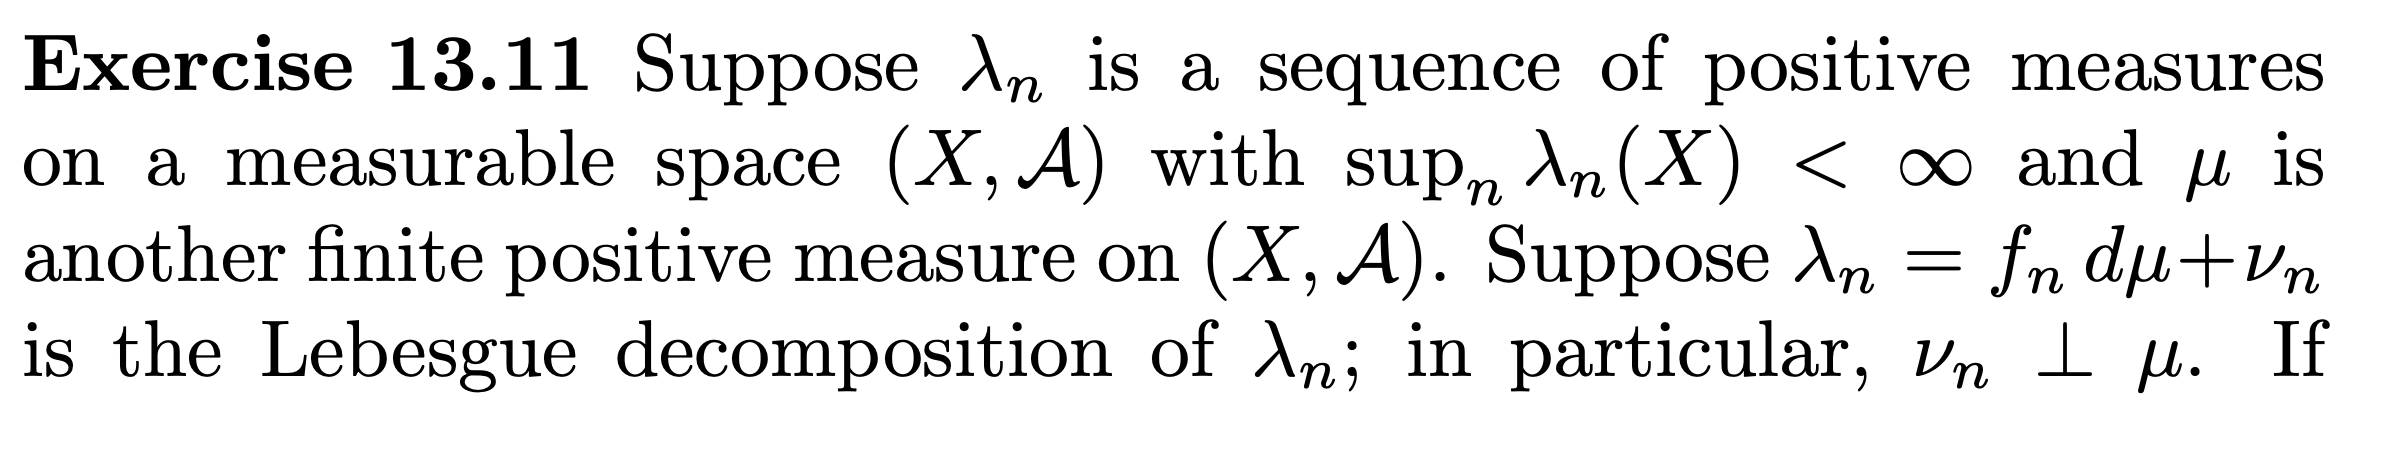
\includegraphics[width=400pt]{img/analysis--berkeley-202a-hw11-c5a4.png}
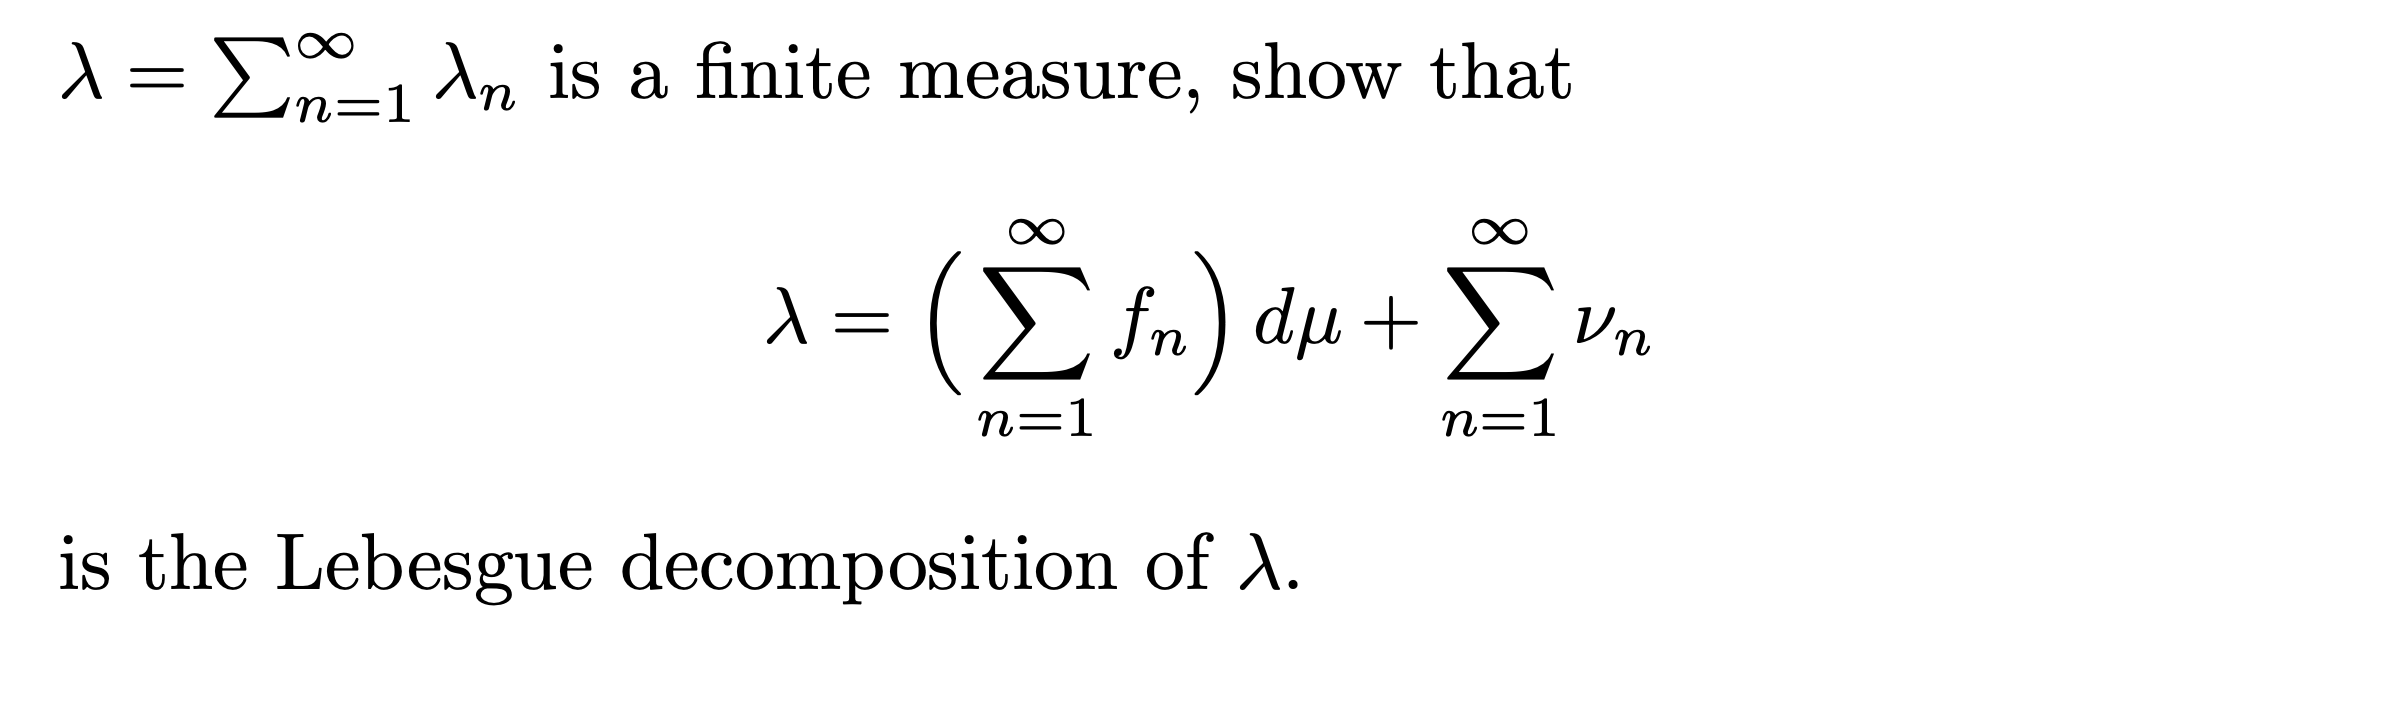
\includegraphics[width=400pt]{img/analysis--berkeley-202a-hw11-3974.png}
\end{mdframed}